\section{Introduction}\label{sec:intro}
In the popular imagination, programmers spend their days interacting with screens of flowing text. 
Textual program editors are powerful and expressive user interfaces, 
so it is little wonder that they remain dominant decades after the teletype. 
However, textual user interfaces are not the best tool for every job. In particular, there are many 
data types for which a non-textual  
user interface is situationally more appropriate. 

For example, consider the following record type\footnote{We will assume that we are in an ML-family language, e.g. Elm (TODO cite), for the remainder of this paper, though the ideas are general.} classifying colors:
\begin{lstlisting}[numbers=none]
type Color = { r: Int, g: Int, b: Int, a : Int }
\end{lstlisting}
It is possible to select a particular color by entering  
an expression of this type using a text editor.
% \begin{lstlisting}[numbers=none]
% let bgcolor : color = { r: 255, g: 178, b: 45, a }
% \end{lstlisting}
The problem is that this \emph{de facto} user interface for color selection offers the user no immediate feedback 
and limited editing affordances. 
It is difficult for the programmer, or anyone subsequently reading the code, to know which color is represented 
and to interactively tweak that color. 
Better supporting these activities would be particularly useful when engaging in live and exploratory programming 
in domains like web design, audiovisual production, and interactive data analysis.

Indeed, practitioners in domains like these commonly turn to   
graphical end-user applications---%
image and video editors, spreadsheets, music composition software, and so on---%
that do provide live feedback and 
direct manipulation affordances. 
The trade-off is that these end-user applications have limited or no support for programmatic abstraction and composition. 
It is difficult, for example, to bind a
color to a variable for use in multiple places, or to darken a color by passing it to a function, or to organize and distribute color schemes using a package manager.
Moreover, it is difficult to compose affordances in ways that the application designer has not 
anticipated, e.g. to use a slider to manipulate the alpha channel of a color 
if the native color palette provides only a text box.

This paper is motivated by the conviction that it is possible to resolve this apparent tension between 
programmatic and direct manipulation by designing a programming system that 
is able to surface GUIs for working with data types for which 
they are useful, while also retaining support for textual program manipulation  
and the full array of abstraction and composition mechanisms
available in modern general-purpose programming languages.

\subsection{Background}
We are not, of course, the first to attempt to integrate   
programming languages and direct manipulation user interfaces. 
Prior work on projectional editing
and active code completion, summarized in Sec. \ref{sec:related-work}, 
has also considered the problem of entering expressions 
of certain types, like \li{Color}, 
using specialized GUIs integrated into a erprogram editor. 
The prior work most closely related to this paper is the {Graphite} system for Java \cite{DBLP:conf/icse/OmarYLM12}.
Graphite allows library providers to associate GUIs, called \emph{palettes}, with types. 
The programming environment offers the programmer the option, via the code completion menu, 
to activate the associated GUI wherever an expression of the corresponding type is needed, 
i.e. wherever there is a \emph{hole} of that type in the program text. 
It is the GUI's job to fill the hole, i.e. to generate an 
appropriate expression to fill the hole. 
Figure~\ref{fig:color}, reproduced from this prior work, demonstrates an example of a simple color chooser.

This prior study extensively evaluated this mechanism. Most notable, the study 
performed a survey of 450 developers and found
that a mechanism of this sort would be valued. The prior work also solicited use cases from these
developers, gather N examples that the authors grouped heuristically into a number of categories. Some examples:

\dots

This paper takes this extensive empirical evaluation as sufficient to establish the utility and broad applicability of a mechanism
of a mechanism of this sort. Our focus in this paper is on addressing a number of non-trivial technical 
deficiencies that limit the ability of library providers to implement useful palettes. 

\begin{figure*}
\begin{center}
\includegraphics[width=35pc]{color_palette.png}\end{center}
\caption{This figure, reproduced from the prior work \cite{DBLP:conf/icse/OmarYLM12}, shows (a) a simple example GUI associated with the \texttt{Color} type, and (b) the code generated by this GUI once the ephemeral interaction is complete.}
\label{fig:color}
\end{figure*}

\begin{figure*}[t!]
\begin{center}
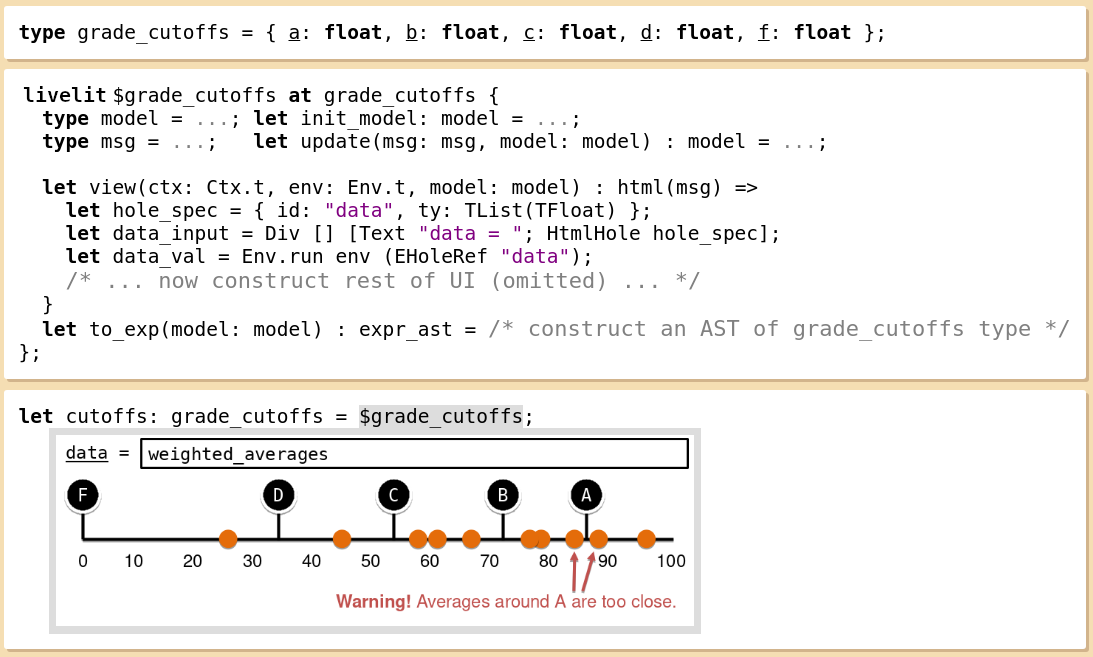
\includegraphics[width=34pc]{cutoffs-mockup.png}\end{center}
\caption{A mockup of a livelit for adjusting grade cutoffs. Livelits are persistent and can access the live environment.}
\label{fig:cutoffs}
\end{figure*}

There are two major limitations with this prior work. 
First, GUIs in Graphite are \textbf{ephemeral}, i.e. they disappear once the initial interaction is complete, leaving behind only the textual representation. This means that feedback and assistance is available only to the programmer
that first writes the code. 
% Graphite does include an \emph{ad hoc} mechanism that allows palettes to parse user-selected code when the GUI loads, but this requires significant additional effort. 

Second, Graphite does not provide any compositional way to {enter subexpressions within the GUI}.
This implies that Graphite's GUIs can only generate \textbf{closed expressions}. For example, in Figure~\ref{fig:color}, there is no way to specify that the \texttt{R}, \texttt{G}, or \texttt{B} values of the color being entered should be computed by a specified expression---only closed colors are supported. 
% This limitation precludes a variety of other perhaps more interesting use cases, e.g. GUIs for entering tabular data where each entry in
% the table is an arbitrary expression of the appropriate type. It also precludes nested composition of GUIs, e.g. a table where some entries are numbers generated by manipulating a slider GUI.


\subsection{Summary of Contributions}
Four things:
1. open extensibility

2. persistent

3. compositional

4. live

Begin in Sec.~2 with an overview using a  case study involving several non-trivial livelits, starting 
from the client's perspective and then considering the livelit provider's perpsective in Sec.~3.

In Sec.~4, we provide a formal account of the mechanism, rooted in Hazelnut Live.

In Sec.~5, we describe some extensions of the core mechanism.

In Sec.~6, we outline our implementation of livelits within Hazel.

In Sec.~7, we describe related work. Finally, we conclude in Sec.~8 with a discussion of 
limitations and future work.



\section{Livelits}
To address these limitations, we introduce live literals, or livelits. Figure~\ref{fig:cutoffs} shows a mockup of the definition and application of a livelit named \li{$grade_cutoffs} for adjusting grade cutoffs, represented as values of  record type \li{grade_cutoffs}. Like textual literal forms (e.g. list literals), livelits are alternative representations of expressions of the associated type \cite{DBLP:journals/pacmpl/OmarA18}. % From the perspective of the remainder of the program, \li{cutoffs} is a value of type \li{grade_cutoffs} like any other.
We are implementing livelits in Hazel (\url{hazel.org}), a live functional programming environment with support for typed holes \cite{popl-paper}. We plan to perform a live demo.




The definition of
the livelit, outlined in Figure~\ref{fig:cutoffs}, follows the Elm architecture,
i.e. there are types representing the abstract model and the messages that the 
GUI generates. Livelits are \textbf{persistent} rather than ephemeral, i.e. the model is recorded in the underlying syntax tree. The \li{view} function generates the GUI, implemented using HTML, on demand (so the view is not persisted). Another function, \li{to_exp}, is responsible for generating the underlying expression, called the \emph{expansion}, from the \li{model}. 
While other projectional editors, e.g. those generated by Citrus \cite{DBLP:conf/uist/KoM05}, also support persistent GUIs in code, they are not user-extensible. 

The GUI can itself contain typed holes, represented by the \li{HtmlHole} constructor. In this case, there is a single hole
for entering an expression of type \li{list(float)}, i.e. the list of weighted
averages. In this example, the user has filled this hole with a variable,
\li{weighted_averages} (the definition of which precedes the content of this figure and is not shown). In other words,
livelits support \textbf{open expressions} and therefore interact cleanly with 
standard abstraction mechanisms, i.e. they can appear under binders. We follow the reasoning principles for literals with spliced sub-expressions established  by \citet{DBLP:journals/pacmpl/OmarA18}.

The main complication when dealing with open expressions relates to how live feedback
is to be generated. Given just the symbolic expression in the hole, it would be 
impossible to plot (as orange dots) the actual data from the list that the variable refers to. To resolve this issue, the system evaluates the program 
as if it the livelits were empty holes, 
relying on the support for evaluating incomplete programs described recently 
by \citet{DBLP:journals/pacmpl/OmarVCH19}. The result of evaluation is an expression containing
hole closures, i.e. holes equipped with environments. 
%Hazel allows the user to interactively select which closure
%interests them if multiple closures for a given hole appear in the result (e.g. if a livelit appears inside a function called multiple times). 
The livelit 
can then evaluate the expression in the hole against the closure selected by the user (not shown) using \li{Env.run}.


%%%%%

\todo{this is the WIP one from last year}{}
Programs are most often represented as text.
%
This representation format provides expert programmers access to a variety of
text editors and text edit actions---to affect fine-grained control over
programming decisions---and a large ecosystem of other text-based
utilities---for example, for line-based file differencing of source code
versions.
%
On the other hand, the flexibility and low-level nature of text comes at some
costs.
%
For experts, some tedious and manual edits could lead to
inefficiency---especially because many routine code editing operations do not
require the full flexibility of text~\citep{XXX}.
%
For novices, the large class of syntax errors that stem from text-edits presents
a steep learning curve.

Motivated to overcome the disadvantages of represent programs as text, a variety
of alternative code editing interfaces have been investigated.
%
At the opposite end of text are \emph{visual programming languages}, which often
completely represent a program with graphical elements~\citep{XXX}.
%
To forgo text completely, such approaches often target domain-specific
languages, such as dataflow programing~\citep{XXX} and pedagogical languages
that are, by design, restricted to relatively few building blocks.
%
Other \emph{structure}, or \emph{projectional} editors, still use a significant
amount of text to render programs, but forgo text-edits in favor of
\emph{structure edit actions} which transform the program (represented as a tree
or some other structure), sidestepping the danger of invalid intermediate states
of concrete syntax.

On the spectrum somewhere between fully text- and fully structure-based are
``hybrid'' editors, which augment text with additional ways to visualize and
manipulate the structure of the program.
%
Victor Scrubbing, APX~\citep{APX}, Sketch-n-Sketch~\citep{sns-pldi}, and Carbide
IDE~\citep{XXX}, among others, allow numeric values to be ``scrubbed'' by
directly manipulating sliders rather than text-editing numeric literals.
%
Barista~\cite{Barista} is a hybrid Java editor where custom \emph{structure
view} GUIs provide alternate representations of expressions instead of text.
%
For example, an arithmetic expression may be rendered with mathematical symbols,
a method may be accompanied by interactive documentation with input-output
examples, and structures may be selectively collapsed, expanded, or zoomed.
%
Graphite~\citep{Graphite} allows custom GUIs---called \emph{palettes}---to help
the programmer fill missing expressions---``holes''---in the program.
%
For example, a color palette can provide visual previews of different candidate
color values, and a regular expression palette can show input-output examples
for different candidate regular expressions.

The GUI representations and interactions enabled by the above hybrid editors are
useful, but several limitations likely preclude wider utility:
%
the types of expressions that benefit from alternative GUI editors are limited
to
%
privileged types that have baked-in interfaces~\citep{XXX}
%
or just of base type~\citep{XXX};
%
the GUI view is ephemeral, in that it disappears once it has been used to
generate an expression~\citep{XXX}; or
%
expressions generated by the GUI are not deeply integrated with the static type
system and interpreter of the language~\citep{XXX,XXX,XXX}.


%% refactoring
%% 
%% DNDRefactoring~\citep{DNDRefactoring}
%% Deuce~\citep{sns-deuce}


\parahead{Persistent, Composable, and Live GUIs for Filling Holes}

compared to the ``simple'' palettes

extend palettes with: persistence, composition, and live feedback

macro systems allow alternative syntactic (i.e. string) representations, to
expand into underlying expressions

palatable

by analogy to these ``literal'' macro systems, palettes are ``graphical
macros'': through interaction with the user, the GUI generates the underlying
expression.

TLMs~\cite{TLMs}


\parahead{Contributions and Paper Outline}


design for palettes. specifically, within the Hazelnut Live framework,
which is a system to address the gap problem that arises in traditional editor
frontends.

demonstration of the expressiveness of the approach through a series of
examples, many of which are drawn from the user study mentioned before.

a prototype implementation of palettes within Hazel, which currently
supports several examples using a core calculus with minimal features. the
implementation provides a clear path for scaling up to larger, full-featured
syntactic programming conveniences, as well as further UI design in future work.

prototype UIs:

  \begin{enumerate}
    \item \Hazel{}: (palette macros;) structure edit actions; expression formula bar; inline layout
    \item \sns{}: (palette functions;) text editor; pop-up menu
  \end{enumerate}

hazelnut~\citep{Hazelnut,HazelnutLive}



